\section{Methodology}

\subsection{System Overview}
The phishing detection system was designed as a meta-model fusion architecture that combines multiple specialized modules instead of relying on a single monolithic classifier. The motivation for this design is that phishing emails expose suspicious patterns across several different information channels, including subject text, body content, sender identity, header structure, and embedded URLs. A single classifier trained on one modality may miss useful evidence available in the others. Therefore, the final system aggregates the outputs of dedicated submodels and learns how to combine them using a supervised fusion layer.

The final pipeline contains five primary modules:
\begin{itemize}
  \item a \textbf{subject module} for subject-line classification,
  \item a \textbf{body module} for message-body classification,
  \item a \textbf{header module} for structural email-header analysis,
  \item a \textbf{URL module} for malicious-link assessment, and
  \item a \textbf{sender module} for phishing detection from sender identity patterns.
\end{itemize}

These module outputs are then passed to a final \textbf{fusion meta-model}, which produces the overall phishing probability.

\subsection{Dataset Construction and Preprocessing}
Two main data sources were used during this work:
\begin{itemize}
  \item an existing cleaned email dataset at \texttt{data/processed/cleaned\_phishing\_dataset.csv}, and
  \item the EPVME email corpus extracted from \texttt{epvme/EPVME-Dataset/extracted}.
\end{itemize}

The EPVME corpus was converted from raw \texttt{.eml} messages into structured CSV form. For each email, the following fields were extracted whenever available:
\begin{itemize}
  \item \texttt{body},
  \item \texttt{url},
  \item \texttt{sender},
  \item \texttt{subject},
  \item \texttt{header},
  \item \texttt{label},
  \item \texttt{source}.
\end{itemize}

To make the combined dataset suitable for super-model training, the following preprocessing steps were applied:
\begin{itemize}
  \item normalization of whitespace,
  \item removal of invalid control characters,
  \item safe UTF-8 sanitization for malformed emails,
  \item normalization of missing values,
  \item extraction and cleanup of URL fields,
  \item removal of duplicate records, and
  \item balancing of the final training set to reduce class skew.
\end{itemize}

The final super-model training dataset was stored as \texttt{dataset/processed/super\_model\_training.csv}. It contains the fields \texttt{sender}, \texttt{subject}, \texttt{body}, \texttt{urls}, \texttt{headers}, \texttt{label}, and \texttt{source}. The balanced dataset contains 34,588 rows, with 17,294 legitimate and 17,294 phishing samples.

\subsection{Individual Detection Modules}

\subsubsection{Subject Module}
The subject module is a text classifier that transforms the email subject line into numerical features using TF-IDF together with hand-crafted subject features such as urgency indicators, exclamation count, capital-letter usage, and length. The module outputs a phishing probability $p_{\text{subject}}$.

\subsubsection{Body Module}
The body module analyzes the email message body. Its preprocessing stage cleans raw email text and extracts stylistic and phishing-related signals such as urgency terms, URL count, uppercase count, punctuation emphasis, message length, and suspicious currency-token usage. The trained body model outputs a phishing probability $p_{\text{body}}$.

\subsubsection{Header Module}
The header module uses the raw email header block and extracts structural security features such as:
\begin{itemize}
  \item multiple \texttt{From:} fields,
  \item mismatches between \texttt{From} and \texttt{Return-Path},
  \item suspicious \texttt{Reply-To} usage,
  \item \texttt{Message-ID} inconsistencies,
  \item \texttt{Received} hop count,
  \item duplicate headers,
  \item freemail-domain usage,
  \item encoded sender or subject values.
\end{itemize}

This module produces a phishing probability $p_{\text{header}}$ and was particularly important in the final model.

\subsubsection{URL Module}
The URL module evaluates extracted links. It uses URL-specific lexical and structural features such as URL length, digit patterns, special characters, shortening services, suspicious domain structure, and malformed syntax. It outputs a phishing probability $p_{\text{url}}$.

\subsubsection{Sender Module}
The sender module was trained specifically on the sender field using character n-gram TF-IDF features and logistic regression. This was necessary because sender identity often contains strong phishing signals such as spoofed domains, unusual formatting, or deceptive naming patterns. The module outputs a phishing probability $p_{\text{sender}}$.

\subsection{Meta-Model Fusion}
The final classifier is a logistic-regression meta-model trained on module-level probabilities and lightweight auxiliary features. Instead of assigning manual weights, the system learns the contribution of each component from data. This is a key methodological advantage of the proposed approach because it allows the fusion layer to discover which evidence sources are most informative.

The final fusion feature vector is:
\[
[p_{\text{subject}},\; p_{\text{body}},\; p_{\text{header}},\; p_{\text{url}},\; p_{\text{sender}},\; has\_url,\; url\_count]
\]

where:
\begin{itemize}
  \item $p_{\text{subject}}$ is the subject-module phishing probability,
  \item $p_{\text{body}}$ is the body-module phishing probability,
  \item $p_{\text{header}}$ is the header-module phishing probability,
  \item $p_{\text{url}}$ is the URL-module phishing probability,
  \item $p_{\text{sender}}$ is the sender-module phishing probability,
  \item \texttt{has\_url} indicates whether at least one URL is present, and
  \item \texttt{url\_count} counts the number of extracted URLs.
\end{itemize}

The final trained fusion model is stored as \texttt{src/models/fusion\_model\_super\_eval.pkl}.

\section{Experimental Output and Results}

\subsection{Generated Report Artifacts}
The evaluation pipeline generated the following artifacts for report use:
\begin{itemize}
  \item confusion matrix values: \texttt{dataset/artifacts/super\_eval/fusion\_confusion\_matrix.csv},
  \item metrics table: \texttt{dataset/artifacts/super\_eval/fusion\_metrics.csv},
  \item coefficient table: \texttt{dataset/artifacts/super\_eval/fusion\_coefficients.csv},
  \item baseline comparison: \texttt{dataset/artifacts/super\_eval/fusion\_baselines.csv},
  \item ablation study: \texttt{dataset/artifacts/super\_eval/fusion\_ablation.csv},
  \item ROC curve: \texttt{graphs/graph\_fusion\_roc\_curve.png},
  \item precision-recall curve: \texttt{graphs/graph\_fusion\_precision\_recall\_curve.png},
  \item confusion matrix figure: \texttt{graphs/graph\_fusion\_confusion\_matrix.png}.
\end{itemize}

\subsection{Final Fusion Model Performance}
The final sender-inclusive fusion model achieved the following results on the held-out test split:

\begin{table}[h]
\centering
\begin{tabular}{lr}
\hline
\textbf{Metric} & \textbf{Value} \\
\hline
Accuracy & 0.9931 \\
Precision & 0.9897 \\
Recall & 0.9965 \\
F1-score & 0.9931 \\
ROC-AUC & 0.9997 \\
PR-AUC / Average Precision & 0.9997 \\
\hline
\end{tabular}
\caption{Final fusion model performance metrics.}
\label{tab:fusion_metrics}
\end{table}

\subsection{Confusion Matrix}
The confusion matrix for the final fusion model is shown in Table~\ref{tab:confusion_matrix}. It indicates that the model made very few errors on the held-out set.

\begin{table}[h]
\centering
\begin{tabular}{lrr}
\hline
\textbf{Actual / Predicted} & \textbf{Legitimate (0)} & \textbf{Phishing (1)} \\
\hline
Legitimate (0) & 3423 & 36 \\
Phishing (1) & 12 & 3447 \\
\hline
\end{tabular}
\caption{Confusion matrix of the final fusion model.}
\label{tab:confusion_matrix}
\end{table}

The corresponding image can be inserted in the report as follows:
\begin{verbatim}
\begin{figure}[h]
  \centering
  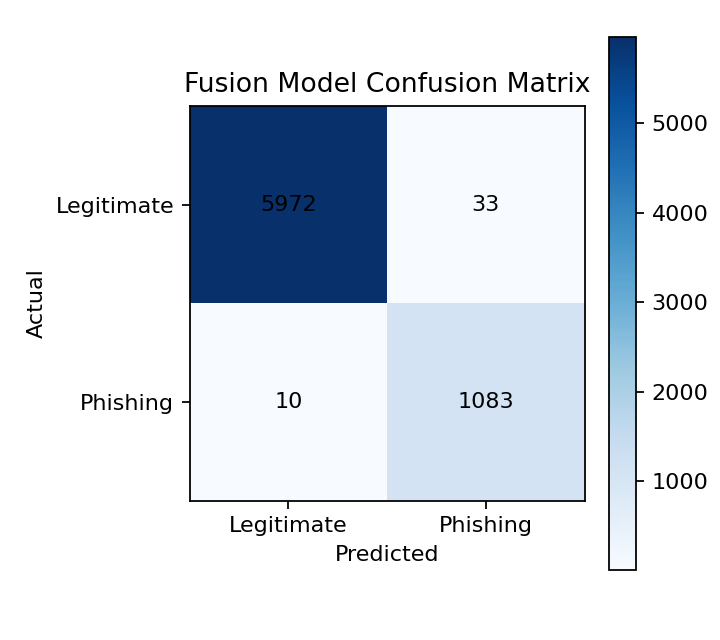
\includegraphics[width=0.55\textwidth]{graphs/graph_fusion_confusion_matrix.png}
  \caption{Confusion matrix for the final fusion model.}
\end{figure}
\end{verbatim}

\subsection{ROC Curve and ROC-AUC}
The ROC curve for the final fused model is stored in \texttt{graphs/graph\_fusion\_roc\_curve.png}. The measured ROC-AUC is 0.9997, which indicates near-perfect ranking ability between phishing and legitimate emails.

\begin{verbatim}
\begin{figure}[h]
  \centering
  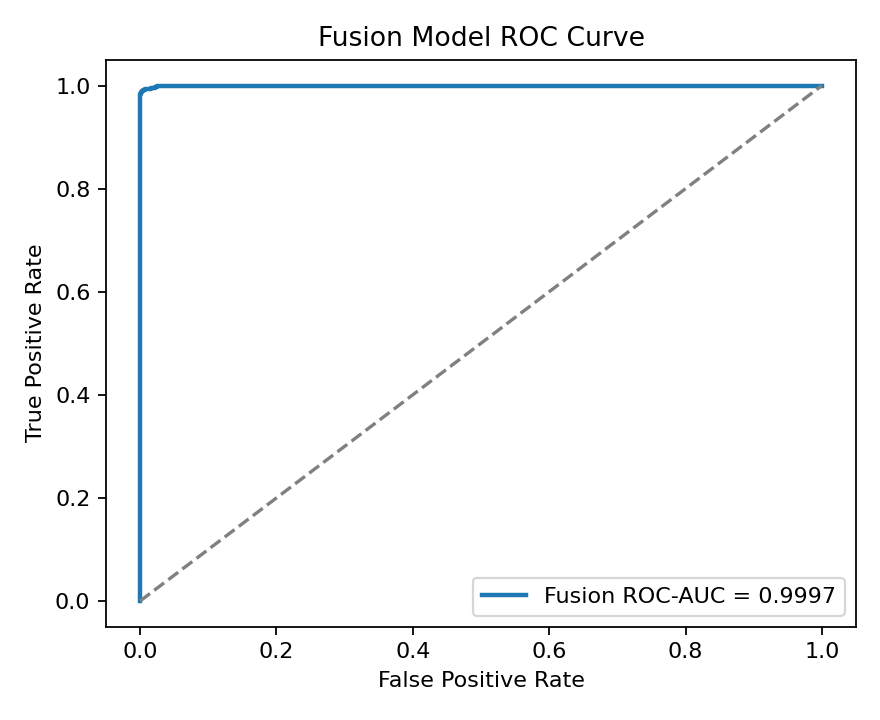
\includegraphics[width=0.62\textwidth]{graphs/graph_fusion_roc_curve.png}
  \caption{ROC curve of the final fusion model.}
\end{figure}
\end{verbatim}

\subsection{Precision--Recall Curve and Average Precision}
The precision--recall curve is stored in \texttt{graphs/graph\_fusion\_precision\_recall\_curve.png}. The average precision score is 0.9997, showing that the model maintains both very high precision and very high recall across thresholds.

\begin{verbatim}
\begin{figure}[h]
  \centering
  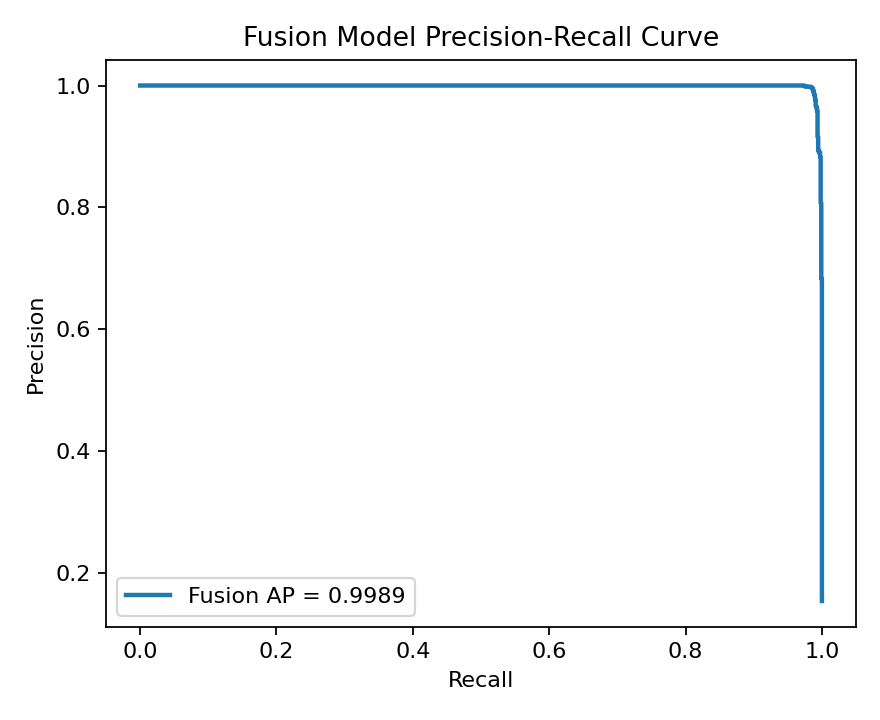
\includegraphics[width=0.62\textwidth]{graphs/graph_fusion_precision_recall_curve.png}
  \caption{Precision--recall curve of the final fusion model.}
\end{figure}
\end{verbatim}

\subsection{Learned Fusion Weights}
One of the main contributions of the proposed system is that fusion weights are not manually assigned. Instead, they are learned by the meta-model. The learned coefficients are shown in Table~\ref{tab:coefficients}.

\begin{table}[h]
\centering
\begin{tabular}{lrr}
\hline
\textbf{Feature} & \textbf{Coefficient} & \textbf{Odds Ratio} \\
\hline
$p_{\text{header}}$ & 13.9394 & 1131848.6247 \\
$p_{\text{sender}}$ & 11.0825 & 65021.5661 \\
$p_{\text{subject}}$ & 5.9117 & 369.3444 \\
$p_{\text{body}}$ & 4.4715 & 87.4899 \\
\texttt{has\_url} & 0.6225 & 1.8636 \\
\texttt{url\_count} & -0.1164 & 0.8901 \\
$p_{\text{url}}$ & -0.8006 & 0.4491 \\
\hline
\end{tabular}
\caption{Learned coefficients of the fusion meta-model.}
\label{tab:coefficients}
\end{table}

These results show that header and sender evidence were the strongest positive contributors in the final system. Subject and body also contributed meaningful predictive value. URL-based features were still useful, but they were weaker than sender and header evidence in this dataset.

\subsection{Baseline Comparison}
To justify the usefulness of the fusion approach, the meta-model was compared against two lightweight baselines:
\begin{itemize}
  \item the best single module,
  \item an equal-weight average fusion strategy.
\end{itemize}

\begin{table}[h]
\centering
\begin{tabular}{lrrrrrr}
\hline
\textbf{Model} & \textbf{Accuracy} & \textbf{Precision} & \textbf{Recall} & \textbf{F1} & \textbf{ROC-AUC} & \textbf{PR-AUC} \\
\hline
Best single module (sender) & 0.9426 & 0.9595 & 0.9243 & 0.9415 & 0.9453 & 0.9686 \\
Equal-weight average fusion & 0.7998 & 1.0000 & 0.5996 & 0.7497 & 0.9965 & 0.9966 \\
Meta-model fusion & 0.9931 & 0.9897 & 0.9965 & 0.9931 & 0.9997 & 0.9997 \\
\hline
\end{tabular}
\caption{Comparison of baselines and final fusion model.}
\label{tab:baselines}
\end{table}

This comparison shows that the learned fusion model substantially outperformed both the best standalone module and the equal-weight strategy. Therefore, the additional complexity of the meta-model is justified by a clear performance gain.

\subsection{Ablation Study}
An ablation study was also conducted by removing one module at a time and reevaluating the fusion system. This helps determine the relative importance of each signal source.

\begin{table}[h]
\centering
\begin{tabular}{lrrrrrr}
\hline
\textbf{Removed Feature} & \textbf{Accuracy} & \textbf{Precision} & \textbf{Recall} & \textbf{F1} & \textbf{ROC-AUC} & \textbf{PR-AUC} \\
\hline
Header & 0.8141 & 0.7473 & 0.9491 & 0.8362 & 0.9496 & 0.9705 \\
Sender & 0.9734 & 0.9748 & 0.9720 & 0.9734 & 0.9965 & 0.9968 \\
Subject & 0.9824 & 0.9771 & 0.9879 & 0.9825 & 0.9984 & 0.9983 \\
Body & 0.9918 & 0.9868 & 0.9968 & 0.9918 & 0.9997 & 0.9997 \\
URL & 0.9928 & 0.9908 & 0.9948 & 0.9928 & 0.9997 & 0.9997 \\
\hline
\end{tabular}
\caption{Ablation study of the fusion model.}
\label{tab:ablation}
\end{table}

The ablation results show that the header module had the largest impact on overall performance. Sender was the second most influential feature group. Subject also contributed noticeably, while body and URL information provided smaller but still positive gains.

\section{Conclusion}
This work demonstrates that phishing-email detection benefits strongly from a fusion-based approach that combines complementary information sources. Instead of depending on a single content classifier, the proposed system integrates subject, body, sender, header, and URL evidence through a learned logistic-regression meta-model.

The final results show that this strategy is highly effective. The model achieved 99.31\% accuracy, an F1-score of 0.9931, ROC-AUC of 0.9997, and PR-AUC of 0.9997 on the held-out evaluation split. The confusion matrix also shows that both false positives and false negatives remained very low.

The coefficient analysis and ablation study provide an interpretable justification for the fusion design. In particular, header- and sender-based signals emerged as the strongest contributors, while subject and body information also improved robustness. URL evidence contributed additional value but was less dominant in the final learned model.

Overall, the experimental results justify the use of meta-model fusion for phishing detection. The approach improves detection performance over both single-module classification and naive equal-weight fusion, while still remaining interpretable through learned coefficients, baseline comparisons, and ablation analysis.

\section{Artifact Summary}
The main files produced for the report are:
\begin{itemize}
  \item \texttt{src/models/fusion\_model\_super\_eval.pkl},
  \item \texttt{src/models/sender\_model\_super\_v2.pkl},
  \item \texttt{src/models/sender\_vectorizer\_super\_v2.pkl},
  \item \texttt{graphs/graph\_fusion\_confusion\_matrix.png},
  \item \texttt{graphs/graph\_fusion\_roc\_curve.png},
  \item \texttt{graphs/graph\_fusion\_precision\_recall\_curve.png},
  \item \texttt{dataset/artifacts/super\_eval/fusion\_metrics.csv},
  \item \texttt{dataset/artifacts/super\_eval/fusion\_confusion\_matrix.csv},
  \item \texttt{dataset/artifacts/super\_eval/fusion\_coefficients.csv},
  \item \texttt{dataset/artifacts/super\_eval/fusion\_baselines.csv},
  \item \texttt{dataset/artifacts/super\_eval/fusion\_ablation.csv},
  \item \texttt{dataset/artifacts/super\_eval/results.md}.
\end{itemize}
